\section{Introduction}
하루에 30만개 이상의 멀웨어가 생성되고 있고 이 숫자는 계속 늘어나고 있다. 같은 기능을 하지만 해시는 다른 멀웨어들을 자동으로 제너레이션 하는 멀웨어 obfuscation 툴들의 발전 및 배포가 그 이유이다. 반면 보안 전문가의 시간은 늘어나지 않고 있다. 보안 전문가는 크게 두 가지 일을 하는데, 하나는 해시로 걸러지지 않은 악성코드의 카테고리를 분류하는 일이고 두 번째는  주요 악성코드에 deep dive 해서 obfuscation 방법이나 악성 행위 방법을 공부하고 후에 나올 악성코드에 잘 대응할 수 있게 하는 것이다.   

이 두 가지 주요 업무 중에서 머신러닝이 쉽게 도움을 줄 수 있는 부분은 두 번째 태스크이다. 사실상 수많은 new 악성코드들을 보안 전문가들이 하나하나 정적 혹은 동적 분석을 통해 분류하는 일은 불가능하다. 따라서 자동으로 멀웨어를 분류하는 시스템은 예로부터 많이 만들었다. PE 스트럭쳐나 콜그래프 등의 정적 피쳐를 받아서 SVM, RF, DNN 등으로 멀웨어를 분류하는 모델이 연구되어왔다.   

하지만 이렇게 만들어진 분류기들에는 문제가 있다. 그 시스템들은 학습된 샘플들에 대해서는 좋은 정확도를 보이지만 새로운 샘플에 대한 대응이 좋지 못하다. 소분류를 레이블로 주고 가르치면 종류가 너무 많고 계속 추가되는 소분류가 지속해서 생긴다. 대분류를 레이블로 주고 가르치면 정적 피쳐 기준 이너클래스 베리언트가 너무 커지고 레이블의 모호성이 발생한다. 따라서 보안 전문가는 멀웨어 분류를 위해 학습된 머신러닝 모델을 사용하고나서 그 결과를 확인해야하는 수고를 해야한다. 그리고 그 확인 과정은 비슷한 멀웨어들을 검색해주는 시스템이 구축되어있지 않다면 오래 걸리게 된다.  

따라서 classification model 을 검증하는데에 사용할 수 있으면서도 동시에 위에서 언급한 보안 전문가의 두번째 태스크인 deep dive 에도 도움을 줄 수 있는 멀웨어 IR System 에 대한 니즈가 증가하고 있다.  
 
기존 멀웨어 IR system 은 크게 LSH나 imphash와 같은 hand-craft Feature representation 을 사용하는 시스템과, ML을 트레이닝시키며 얻은 automatically extracted feature representation 을 사용하는 시스템이 있다. 전자의 장점은 False Negative 가 낮다는 것이지만, generalization 이 잘 안된다는 단점이 있다.[] 더 좋은 generalization 을 위해 후자의 기법들이 개발되었지만, 멀웨어 representation location 이 사람의 시멘틱 스페이스와 어긋나있다는 단점이 IR 결과의 정상 평가 결과(?)를 낮추고 있다.   

우리는 이러한 문제들을 해결하고 사람의 인지스페이스와 멀웨어 임베딩 스페이스가 동기화되어있는 멀웨어 IR 시스템을 제안한다. 또한 우리는 멀웨어 인포메이션 리트리벌 시스템을 만들 때의 어려운 점들과 그 문제들을 어떻게 해결했는지를 설명한다. 그리고 쿼링 결과를 시각적으로 보여서 우리의 인지와 임베딩 스페이스가 얼마나 동기화되어있는지 확인한다.  

페이퍼 구성은 다음과 같다: related work 가 섹션 2에 위치한다. 섹션 3은 우리가 풀고자하는 문제를 정의하고 어떤 IR 시스템이 좋은 시스템인지에 대한 이야기를 한다. 섹션 4은 우리가 제안하는 malware IR 시스템의 디자인과 구현 과정을 설명한다. 구현 과정에는 크게 두 페이즈가 있는데 첫 째는 섹션 5에서 설명할 임베딩 학습 페이즈이고 둘 째는 섹션 5에서 설명할 리트리벌 페이즈이다. 섹션 6에서는 실험에 쓰인 뉴럴넷과 데이터셋,그리고 실험 결과에 대해서 설명하고 임베딩 벡터를 시각화한다. 섹션 7에서는 Future works 그리고 세션 8 에서는 결과를 보여준다. 


\section{Related Works}


Nataraj et al. \cite{nataraj2013sarvam} proposed a large scale malware search and retrieval system. In this paper, he proposes a method to retrieve fingerprints from malware image and retrieves similar samples through nearest neighbor search. Upchurch et al. \cite{upchurch2015variant} introduced a framework for detecting variant malware through similarity testing. This framework extracted the static features using BitShred, TLSH, sdhash, ssdeep, and compared them to determine whether they were similar malware. Palahan et al. \cite{palahan2013extraction} proposed a method of comparing similarities between malware by extracting significant malicious behaviors from the system call dependency graph and comparing them. Several neural IR models have been proposed in the document retrieval domain, and many models have been studied to obtain a good representation of text\cite{mitra2017learning,cohen2016end,huang2013learning}.

 Chih-Kuan et al. \cite{yeh2017learning} trained Canonical Correlated AutoEncoder models using label-correlation sensitive loss function as a way to obtain multilabel embedding. In this paper, he showes that the relationship between labels with dependency is trained end-to-end and solves the multi-label classification task, and proved to be effective for missing label problem of multilabel classification.

\section{Problem Settings}

우리가 제안하는 malware IR 시스템은 벡터 학습 과 리트리벌 두 페이즈로 나뉜다. 두 페이즈에서 사용될 노테이션들을 정의하고, 이들을 이용해서 각 페이즈에서 어떤 태스크를 행해야하는지를 설명한다. 

\subsection{Notations}

우리는 먼저 학습 멀웨어 셋으로 Y를 갖고 있다. 그리고 각 멀웨어에 해당하는 싱글레이블 셋  Ys 과 멀티레이블 셋 Ym 이 있다. 이 레이블을 얻는 방법은 섹션 6.1에서 자세히 설명한다. 그리고 각 멀웨어로부터 손으로 추출된 피쳐의 튜플들의 셋을 V 로 정의한다. 어떤 피쳐들을 추출해서 사용했는지는 섹션 6.2에서 설명한다. 

멀웨어 IR 시스템은  4개의 원소를 갖는 tuple 로 정의된다. h 는 멀웨어 피쳐로부터 벡터 representation 을 얻을 수 있는 임베더 함수이다. E 는 검색이 될 멀웨어의 임베딩 벡터 셋이다. d 는 입력된 쿼리와 임베딩 벡터 간 거리를 계산하는 함수이다. R 은 리트리벌 결과를 반환하는 프레임워크이다. 학습 페이즈에서는 적절한 h 를 학습하고 이를 통해 Z로부터 E를 얻는다. 리트리벌 페이즈에서는 멀웨어 샘플 쿼리 q 를 입력받고 가장 가까운 k 개의 neighbor 를 랭킹 모듈 R 을 통해 반환한다.


\subsection{Tasks}

학습페이즈에서는 IR system 에서 사용하기 위한 벡터 리프레젠테이션을 얻기 위한 Auxiliary Task를 수행한다. Auxiliary Task 는 멀웨어 분류 태스크를 학습하는 것으로 싱글 레이블 클래시피케이션이나 멀티레이블 클래시피케이션이 될 수 있다. f 인 f 는 멀웨어 피쳐로부터 레이블을 추정하는 함수이다. 함수 f 는 다시 g 와 h 의 합성 함수로 정의할 수 있다. h 는 위에서 설명한, 멀웨어 피쳐로부터 vector representation 을 얻을 수 있는 임베딩 함수이다. g는 임베딩으로부터 label 을 추정할 수 있는 클래시파이어이다.  
f(Z)

리트리벌 페이즈에서는 멀웨어 샘플 쿼리 q를 입력받아 학습 페이즈에서 구했던 h 함수를 이용하여 임베딩한다. 임베딩된 쿼리 eq 와 E 의 원소들 간 거리를 d 함수를 통해 측정하고, 가까운 k 개의 neighbor 를 랭킹 모듈 R 을 통해 반환한다. 
Result tuples = (Xvecj ) where



\section{Malware Information Retrieval System}
% 목표하는 바
이번 세션에서는 제안된 malware information retrieval system 의 동작과 구성 그리고 가져야하는 속성들을 설명한다. 우리의 시스템은 크게 학습과 검색(retrieval), 두 페이즈로 나뉜다. 학습 페이즈에서는 원할한 검색을 위해 시멘틱스를 반영하는 학습 데이터의 표현 벡터를 학습한다. 검색 페이즈에서는 유저로부터 입력된 멀웨어 혹은 태그 쿼리와 미리 저장해놓은, 학습된 표현 벡터들로부터 랭킹 결과를 출력한다. 이어지는 서브 섹션에서는 두 페이즈에서 사용될 노테이션들을 정의하고, 이들을 이용해서 각 페이즈에서 어떤 태스크를 행해야하는지를 자세히 설명한다.  


\subsection{Notations}
우리는 먼저 학습 멀웨어 셋으로 $X = \{x_1, x_2, ..., x_N\}$ 를 갖고있다. 그리고 각 멀웨어에 해당하는 싱글레이블 셋 $Y_s = \{y_{s1}, y_{s2}, ..., y_{sN}\}$ 과 멀티레이블 셋 $Y_m = \{\vec{y}_{m1}, \vec{y}_{m2}, ... , \vec{y}_{mN}\}$ 이 있다. 이 레이블을 얻는 방법은 섹션 6.1에서 설명한다. 그리고 각 멀웨어로부터 손으로 추출된 피쳐들의 셋을 $V = \{v_1, v_2, ..., v_n \}$ 로 정의한다. 

멀웨어 IR 시스템은 $[h, E, d, R]$ 4개의 원소를 갖는 tuple 로 정의된다. $h$ 는 멀웨어 피쳐로부터 벡터 representation 을 얻을 수 있는 임베더 함수이다. $E$ 는 검색이 될 멀웨어의 임베딩 벡터 셋이다. $d$ 는 입력된 쿼리와 임베딩 벡터 간 거리를 계산하는 함수이다. $R$ 은 랭킹 모듈이다. 학습 페이즈에서는 적절한 $h$ 를 학습하고 이를 통해 $V$로부터 $E$를 얻는다. 리트리벌 페이즈에서는 멀웨어 샘플 쿼리 $q$ 를 입력받고 가장 가까운 $k$ 개의 neighbor 를 랭킹 모듈 $R$ 을 통해 반환한다.

\begin{table}[!htb] % notation
\caption{Notations}
\label{tab:notation}
\begin{minipage}{\columnwidth}
\begin{center}
\begin{tabular}{ll}
\toprule
Meaning & Notation\\
\midrule
  Set of malwares     & $X$ \\
  ith malware sample  & $x_i$ \\
  Set of single labels & $Y_s$ \\
  Single label of ith malware    & $y_{si}$ \\
  Extracted features of ith malware & $v_i$ \\
  Set of extracted features   & $V$ \\
  Set of multilabels   & $Y_m$ \\
  Multilabels of ith malware & $\vec{y}_{mi}$\\
  Neural embedder & $h$ \\
  Parameters of neural embedder & $\theta$ \\
  Classifier & $g$ \\   
  Parameters of classifier & $W$, $b$ \\  
  Set of Embedded malware vectors & $E$ \\
  Embedded malware vector & $e$ \\
  Importance coefficient & $c$ \\
  Distance measuring function & $d$ \\
  Semantic component vector & $s$ \\
  Ranking Module & $R$\\
\bottomrule
\end{tabular}
\end{center}
\bigskip\centering
\end{minipage}
\end{table}


\subsection{Tasks}
학습페이즈에서는 IR system 에서 사용하기 위한 벡터 리프레젠테이션을 얻기 위한 Auxiliary Task를 수행한다. Auxiliary Task 는 멀웨어 분류 태스크를 학습하는 것으로 싱글 레이블 클래시피케이션이나 멀티레이블 클래시피케이션이 될 수 있다. $f: V \rightarrow Y $ 인 f 는 멀웨어 피쳐로부터 레이블을 추정하는 함수이다. 함수 $f$ 는 다시 $g$ 와 $h$ 의 합성 함수로 정의할 수 있다. $h$ 는 위에서 설명한, 멀웨어 피쳐로부터 vector representation 을 얻을 수 있는 임베딩 함수이다. $g$는 임베딩으로부터 label 을 추정할 수 있는 클래시파이어이다. 시멘틱을 내포하는 임베딩 벡터를 학습시키는 방법에 대해서는 섹션4에서 자세히 이야기한다. 
\[
f(v_i) = (g \circ h)(v_i) = g(h(v_i)) = g(e_i) = y_i 
\]
where
\[
g(e_i) = \sigma (W*e_i + b) 
\]
% sigma == sigmoid or softmax
리트리벌 페이즈에서는 멀웨어 샘플 쿼리 q를 입력받아 학습 페이즈에서 구했던 h 함수를 이용하여 임베딩한다. 임베딩된 쿼리 eq 와 E 의 원소들 간 거리를 d 함수를 통해 측정하고, 가까운 k 개의 neighbor 를 랭킹 모듈 R 을 통해 반환한다. 

% Algorithm 으로 대체
\[
Results = \{x_j | j = argmin_i( {-d(e_q, e_i)} )  \}
\]


\subsection{Modules}
두 페이즈의 구조도는 Figure 과 같다. 두 페이즈에서 공통으로 존재하는 모듈은 Feature Extractor와 Neural Embedder 가 있다. 벡터 학습 페이즈에는 Classifier 가, 리트리벌 페이즈에는 랭킹 모듈이 포함되어있다. 

\begin{figure}[!htb] % train_phase
  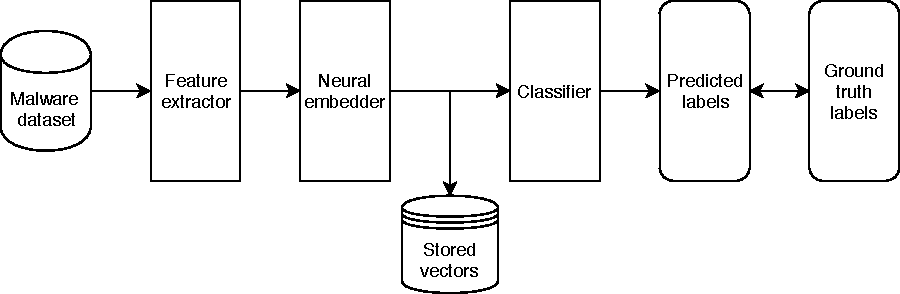
\includegraphics[width=\linewidth]{../figures/train_phase.pdf}
  \caption{train phase}
  \label{fig:train_phase}
\end{figure}

\begin{figure}[!htb] % retrieval_phase
  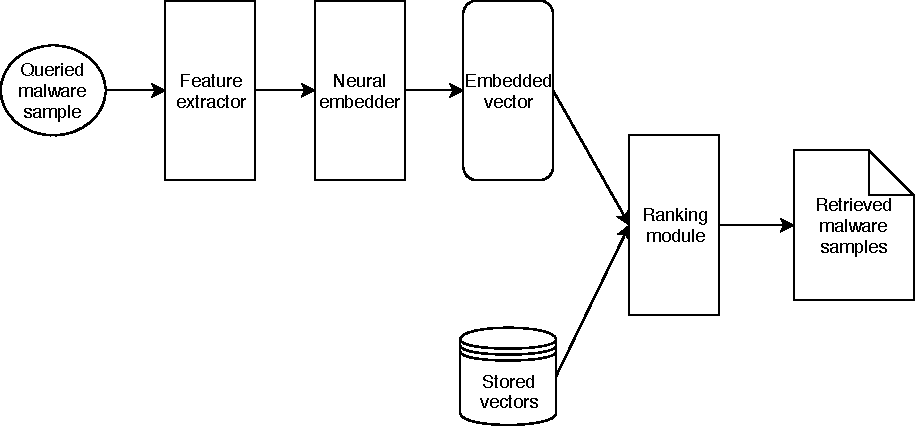
\includegraphics[width=\linewidth]{../figures/retrieval_phase.pdf}
  \caption{retrieval phase}
  \label{fig:retrieval_phase}
\end{figure}

\textbf{Feature Extractor. }
Feature extractor 는 Malware Rawdata 로부터 Handcrafted feature 를 추출하는 모듈이다. Handcrafted feature로 PE 같은경우에는 Size 와 Entropy, Histogram of API Calls, … 등을[*] 추출한다. APK 같은 경우에는 추가적으로 Permission,  … 등의 피쳐를 추출한다. 

\textbf{Neural Embedder. }
Neural embedder 는 Feature extractor 모듈에서 추출된 멀웨어의 피쳐들로부터 Representation vector 를 뽑는 모듈이다. theta 로 Parameterized 되어있는 뉴럴 네트워크이며, 파라미터는 벡터 학습 페이즈에서 Auxiliary Task 를 수행하면서 Optimize 된다. 그리고 리트리벌 페이즈에서 파라미터는 freeze 되어 업데이트되지 않는다. 
Neural Embeder 의 네트워크 구조는 CNN을 사용하였다. Thumbnail 을 받아서 CNN 5 층과 fully 2 층을 쌓은 구조를 사용한다. feature 의 성격에 따라 다른 네트워크 구조로 임베딩 피쳐벡터를 추출함으로써 더 나은 generalization 성능을 얻을 수 있다. thumbnail 피쳐는 [malimg 논문 인용] 악성 코드영역 혹은 악성코드를 특징짓는 영역의 로컬리 시프트 인베리언트한 특성을 담기 위해 CNN 을 사용해서 임베딩 피쳐벡터를 추출한다. 

\textbf{Classifier. }
%% Figure
%\begin{figure}
%  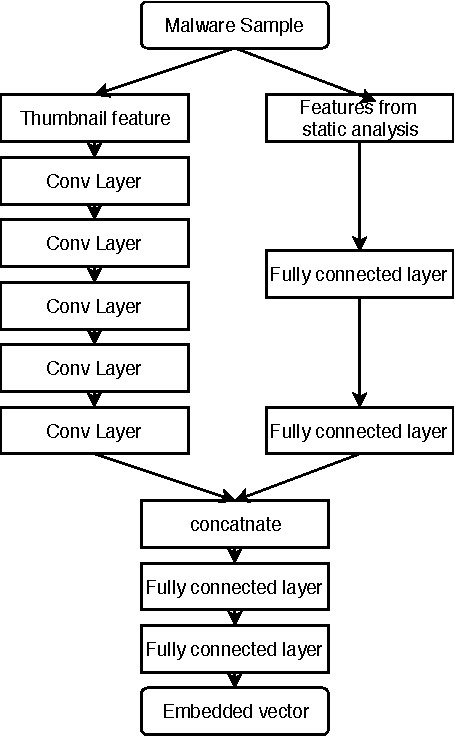
\includegraphics[height=10cm]{../figures/neural_embedder.pdf}
%  \caption{neural embedder}
%  \label{fig:three}
%\end{figure}
Classifier 모듈은 Neural embedder 를 통과해서 나온 embedding vector 를 받아서 각 레이블 별 확률을 출력해준다. 1층의 fully connected 로 파라미터라이즈드 되어있으며 태스크에 따라 softmax 혹은 sigmoid Activation을 사용하였다. Neural Embeder 모듈과 마찬가지로 벡터 학습 페이즈에서 back propagation 에 의해 파라미터들이 학습되고, 리트리벌 페이즈에서는 프리즈된다. 

\textbf{Ranking Module. }
학습 페이즈에 저장해두었던 학습 셋의 임베딩 벡터들과 추출된 벡터의 거리를 거리함수 d 를 사용하여 측정하고 k 개의 nearest neighborhood 를 가까운 순서대로 정렬하고 출력한다.


\subsection{Desired properties}
멀웨어 IR 시스템은 한계들이 존재했다. 특히 Raw binary file 로부터 좋은 피쳐를 뽑기가 수월하지 않고, intraclass variance 는 크고 innerclass variance 는 작으며 계속해서 변종과 새로운 종이 생겨나는 멀웨어 도메인의 특징으로 말미암아 좋은 멀웨어 IR 시스템이 가져야 할 속성들은 다른 도메인의 IR 시스템과는 조금 다르다.

\textbf{Semantic understanding. }
쿼링 샘플에 대해 구조적으로 비슷한 샘플 뿐만 아니라 의미적으로도 비슷한 샘플들을 랭킹하고 retrieve 할 수 있어야 한다. 여기서 의미가 비슷하는 것은 멀웨어의 행동 혹은 사람이 생각하기에 중요한 멀웨어의 속성들이 비슷하다는 것을 의미한다. 구조적으로 다르다고 해도 멀웨어의 행위가 일치하면 같은 의미를 갖는 샘플이라고 볼 수 있다. 마찬가지로 구조적으로 거의 같다고 해도 멀웨어의 행위가 전혀 다르다면 두 샘플은 다른 의미를 가졌다고 할 수 있다. 더불어 우리는 Locky 와 Cerber 라는 두 랜섬웨어 패밀리에 해당하는 샘플 간 유사도가 Locky 와 Coinminer 에 해당하는 두 샘플의 유사도보다 더 작다고 생각한다. 이러한 샘플들 간 의미 차이 까지 고려될 수 있다면 그 시스템은 Symantics-aware한 시스템이라고 할 수 있다. 
 
\textbf{Robustness to novel samples. }
멀웨어의 새로운 변종들은 계속해서 나타나기 때문에 이에 빠르게 대응할 수 있어야 한다. 
%
%\textbf{Robustness to rare inputs. }
%멀웨어 도메인에서의 샘플 수는 그 멀웨어 패밀리의 영향력을 의미하지 않는다. 물론 비례하는 경향이 없는것은 아니지만, 하나의 멀웨어가 전세계적으로 유행할 수도 있고, 변종은 많지만 별로 영향력이 없는 멀웨어일 수도 있다. 따라서 해당 패밀리의 샘플 수가 적다고해서 쿼링 결과에서 랭킹 순위가 밀려서는 안된다. 즉 적은 수의 샘플에 대해서도 모델은 강건해야한다. 

%\textbf{Robustness to variable size inputs. }
%멀웨어의 raw file size Variance 는 매우 크다. 작게는 몇키로바이트부터 크게는 기가단위까지 갈 수 있다. 사이즈에 상관없이 retrieve 를 할 수 있어야 한다.

\textbf{Efficiency. }
세상에 존재하는 멀웨어 샘플 개수는 매우 많고 기하급수적으로 늘어나고 있다. 따라서 수많은 샘플들에서 k 개의 상위 랭크된 결과를 적절한 시간 내에 retrieve 하려면 랭킹 모듈이 효율적이어야한다.






\section{Design and Implement of Malware IR System}

두 페이즈의 구조도는 Figure 과 같다. 두 페이즈에서 공통으로 존재하는 모듈은 Feature Extractor와 Neural Embedder 가 있다. 벡터 학습 페이즈에는 Classifier 가, 리트리벌 페이즈에는 랭킹 모듈이 포함되어있다. 
% Figure
\begin{figure}
  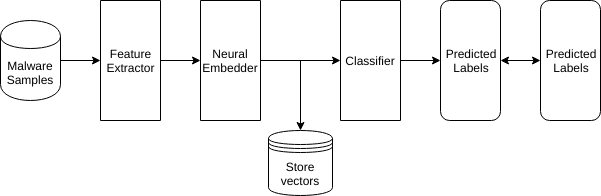
\includegraphics[width=\linewidth]{../figures/train_phase.png}
  \caption{train phase}
  \label{fig:one}
\end{figure}
% Figure
\begin{figure}
  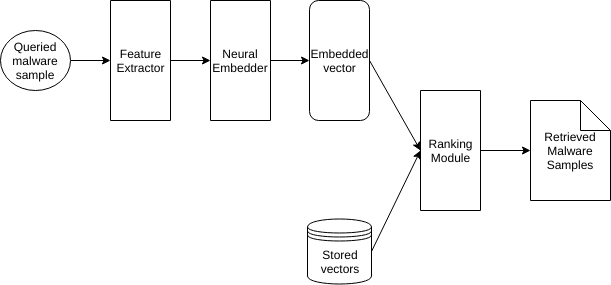
\includegraphics[width=\linewidth]{../figures/retrieval_phase.png}
  \caption{retrieval phase}
  \label{fig:two}
\end{figure}


\subsection{Feature Extractor}

Feature extractor 는 Malware Rawdata 로부터 Handcrafted feature 를 추출하는 모듈이다. Handcrafted feature로 PE 같은경우에는 Size 와 Entropy, Histogram of API Calls, … 등을[*] 추출한다. APK 같은 경우에는 추가적으로 Permission,  … 등의 피쳐를 추출한다. 


\subsection{Neural Embedder}
Neural embedder 는 Feature extractor 모듈에서 추출된 멀웨어의 피쳐들로부터 Representation vector 를 뽑는 모듈이다. theta 로 Parameterized 되어있는 뉴럴 네트워크이며, 파라미터는 벡터 학습 페이즈에서 Auxiliary Task 를 수행하면서 Optimize 된다. 그리고 리트리벌 페이즈에서 파라미터는 freeze 되어 업데이트되지 않는다. 

\subsection{Classifier}

classifier





\section{Auxiliary Task}


\subsection{Single label classification}
Single label classification 딥러닝 모델로 만든 Malware IR System 
장점 : 임베딩된 벡터 representation 에 대해 kNN 해서 IR 이 가능하다.
한계 : 사실 같은 상위카테고리인데 멀리 임베딩된다.
해결법 : 멀티레이블 쓰

\subsection{Multi label learning}
Multi label classification 딥러닝 모델로 만든 Malware IR System 
장점 : 같은 대분류 내의 소분류 애들이 비슷한 곳에 임베딩된다. 
한계: inner class variance 가 너무 커서 IR 할 때 distance 계산 시 노이즈가 발생한다.
해결법 : 메트릭러닝인 센터로스를 쓰자


\subsection{Mutli label centerloss classification}
장점: innerclass variance 가 줄고 interclass variance 가 늘어난다.
한계: 태그 간 관계가 사람의 인지와 다르다
해결법 : 태그 간 중요도를 Constraint 로 넣자

\subsection{Mutli label weighted centerloss classification}
Mutli label classification + weighted centerloss 딥러닝 모델로 만든 Malware IR System 
장점: 태그간 관계가 사람의 인지와 같다. IR 결과가 사람이 생각하는 것과 같이 나온다.


\section{Retrieval Phase}
리트리벌 페이즈에서는 속도와 효율성이 중요하다. 우리 시스템은 저장된 임베딩 벡터들에 대해 거리를 모두 알아야 하므로 저장 개수가 많을 수록 느려지고, 이를 해결하기 위해서 KNN 대신에 ANN 을 사용하였다.  % 좀더서술.

\section{Experiments}

\subsection{Datasets}
모델의 학습과 평가에 사용된 dataset은 VirusTotal로부터 crawling된 샘플 PE 5만여개와 APK 8만여개 중 security expert가 검수하여 확진을 내린 PE 샘플 2천여개 k종의 family, APK 샘플 2만여개 l종의 family로 구성하였다.
또한 VirusTotal에서 제공하는 수십개 이상의 AntiVirus 엔진의 탐지결과로부터 Labeling을 자동화 하였다. VirusTotal로부터 각 AntiVirus 엔진들이 탐지해낸 결과를 의미있는 word 단위로 파싱하고, 샘플들로 부터 얻어진 word token들을 대상으로 security expert가 의미있는 토큰과 그렇지 않은 토큰을 선별하는 작업을 수행하였다. 추가로, 의미 있는 토큰에 대해 중요도에 따라 우선순위를 매기도록 하였다. 이를 통해 학습 샘플에 대해 expert가 일일히 수동으로 label을 다는 시간을 줄이면서도 높은 accuracy의 label을 얻을 수 있다. 또한, 하나의 샘플에 single label이 달릴 때에 비해 multi label을 사용 할 경우 악성코드의 다양한 행위 특성을 반영하도록 모델을 학습 시킬 수 있다. 


\subsection{Hyperparameters}


\subsection{Results}

표 : Performance measures of Malware IR Systems

metric performance measures: acc, auc, tf-idf of labels(?)

row : 기존 방법들, single, multi, weighted multi
col : single-label classification accuracy, multilabel classification auc

non-metric performance measure : top query results

querying results sorted by distances

\subsection{Visualization}

semantic synchronization level

Visualization of representations






\section{Future Works}

현재 방법은 멀티 레이블이 다 정확해야 한다. 아니라면 모델이 noise 로부터 오해를 쉽게 한다. 하지만 이 도메인에서 정확한 레이블을 얻기란 쉽지 않다. 따라서 label noise-robust MLC 를 만들어 멀웨어의 feature 로부터 멀웨어 샘플의 리얼 레이블을 denoising 을 통하여 추정하고, 이를 통해서 IR 시스템을 만든다면 더 semantic-aware 한 Malware Information System 을 만들 수 있을 것이라 추정된다.
더불어 새로운 샘플에 대한 빠른 대응도 IR 시스템에서 중요한 부분인데, 딥러닝 모델이다보니 학습해야할 시간이 필요하다. continual learning 혹은 online update 를 사용해서 이를 해결하는 것도 우리의 Future work이다. 





\section{Conclusions}

우리는 딥러닝을 활용하여 멀웨어 리트리벌 시스템을 만드는 데에서 생겼던 문제들을 새로운 로스를 정의함으로써 해결했다. 특히 기존 방법들보다 [제너럴라이제이션] 측면에서 좋다는 것을 정량적, 시각적으로 증명했다. 이는 수많은 보안 전문가들의 업무 코스트를 낮춰줄 수 있을 것이라 믿는다.

\appendix

\section{Location}

Note that in the new ACM style, the Appendices come before the References.


\begin{acks}
% TODO: For the submission, don't include acknowledgments since they would most likely deanonymize you.
\end{acks}
